
\chapter{Estado del arte}\label{cap:edoarte}

%Que se está utilizando en la literatura o en el mercado para implementar tableros de datos
%Hablar de software Open Source y de paga mencionando ventajas y desventajas de cada uno. También explicar porque cada software no es viable para la solución.

El presente capítulo tiene como objetivo realizar una revisión crítica y sistemática de la literatura y el mercado actual en torno a la implementación de tableros de datos. Se analizará el uso de software \textit{Open Source} y de pago, considerando sus ventajas y desventajas, con el fin de determinar la mejor opción para la implementación de un tablero de datos en el contexto del presente trabajo.\\

Se presentará una revisión de las principales herramientas \textit{Open Source} disponibles para la creación de tableros de datos, como Tableau Public, Google Data Studio y Grafana. Se describirán sus características, ventajas y desventajas. De manera similar, se analizarán las principales herramientas de pago disponibles para la creación de tableros de datos, como Microsoft Power BI, Tableau y Domo.



\section{Software para tableros de datos}\label{sec:seccion3.1}
Un software para la implementación de tableros de datos, es una plataforma centralizada que permite a las empresas e instituciones visualizar y analizar información compleja de forma simplificada e intuitiva. Ayudan a presentar los datos en un formato visualmente atractivo e interactivo, lo que permite a los usuarios supervisar los indicadores clave de rendimiento \textit{(KPI)} y obtener información procesable para tomar decisiones informadas.

En esencia, este tipo de software actúa como puente entre los datos brutos y la información significativa. Transforma conjuntos de datos complejos en representaciones visuales comprensibles. Esto facilita a los usuarios la comprensión e interpretación de la información. Los tableros suelen consistir en diagramas, gráficos, tablas y otros elementos visuales que condensan grandes volúmenes de datos en visualizaciones concisas y significativas. \\

Las principales características que se buscan en un software para el desarrollo de tableros son las siguientes:

\begin{enumerate}
    \item \textbf{Plantillas de tableros predeterminadas y opciones de estilos:} Esta característica permite a los usuarios elegir entre plantillas prediseñadas y personalizar el estilo del tablero para adaptarlo a sus necesidades.
    
    \item \textbf{Seguridad de los datos:} Este es un aspecto importante a tener en cuenta antes de elegir la herramienta adecuada. Garantizar que los datos confidenciales de la institución están protegidos en todo momento es de gran importancia, no sólo por razones de seguridad, sino también porque las normativas de seguridad son cada vez más estrictas.
    
    \item \textbf{Procesamiento de datos en tiempo real:} Un tablero tiene como uno de sus propósito proporcionar las tendencias generales al tiempo que permite a los usuarios la capacidad de desglosar y acceder a múltiples capas de datos.
    
    \item \textbf{Personalización e integración:} Un tablero que puede ser personalizable permite a los usuarios elegir qué puntos de datos y visualizaciones pueden ver, mientras que la integración con otras herramientas permite mejorar los análisis e informes.

    
    \item \textbf{Gráficos:} Un buen software para desarrollo de datos debe de proporcionar gráficas personalizables que ayudan a transmitir las métricas esenciales de forma rápida y atractiva.

    \item \textbf{Opciones para compartir:} Un buen software suele proveer diversas opciones para compartir tableros entre diferentes personas. Esto se puede hacer mediante el inicio de sesión desde otro dispositivo, el envío de tableros e informes por correo electrónico, o el uso de un visor externo.

    \item \textbf{Capacidad de exportación e impresión:} Esta característica permite poder exportar los tableros en archivos con formato PDF o PNG sin que el tablero pierda su estructura y diseño al momento de la conversión.
    
    
\end{enumerate}





\section{Software Open Source}
La implementación de tableros de datos utilizando tecnología de código abierto tiene muchas ventajas que los convierten en una opción sustentable para muchas organizaciones. A continuación se analizarán algunas de los principales software \textit{open source} que se utilizan para la creación tableros de datos creados con tecnología de código abierto, junto con ejemplos de algunos de los principales casos de uso para los que se ha utilizado dicha tecnología.

\subsection{Tablueau Public}
Tableau Public es una plataforma gratuita para explorar, crear y compartir públicamente tableros para la visualización de datos en línea. Cualquier persona puede crear tableros utilizando la aplicación web.\\
Se pueden procesar datos en diversos formatos, como Excel, CSV y Google Sheets, para crear visualizaciones atractivas e interactivas con una interfaz fácil de usar la cual no requiere de la producción de código.\\

La razón principal por la cual esta opción no es viable para la implementación de este proyecto, se debe a que los datos pueden ser observados por cualquier persona, lo cual no de debería ser posible ya que se manipulan datos privados y delicados que no son de uso público.

\subsection{Grafana}
Grafana es una aplicación web de análisis y visualización interactiva multiplataforma. Proporciona tablas, gráficas y alertas para la web cuando se conecta a fuentes de datos compatibles. Es principalmente una herramienta de visualización que proporciona gráficos interactivos para administradores y tableros de datos alimentados por flujos de entrada de datos.\\
Grafana cuenta con un modelo de fuente de datos conectable que puede conectarse con una amplia gama de fuentes de datos, incluidos datos de series temporales, pero también bases de datos relacionales como lo MySQL y PostgreSQL.\\

La razón por la cual se descartó su uso para este proyecto se debe la curva de aprendizaje es grande. La configuración de los plugins puede requerir un esfuerzo considerable. Las opciones de configuración a través de la interfaz gráfica de usuario son limitadas y a menudo es necesario el mantenimiento y la edición manual de los archivos de configuración.


\subsection{Google Data Studio}
Google Data Studio es una herramienta de \textit{Business Intelligence (BI)}, que procesa datos brutos en información estratégica para las empresas e instituciones. A través de la visualización de datos, Google Data Studio reúne métricas e indicadores que apoyan la toma de decisiones y estrategias. Está diseñada para ayudar a los profesionales del marketing, a los propietarios de empresas y a los analistas de datos a visualizar los datos para obtener información y tomar decisiones fundamentadas. Google Data Studio es compatible con más de 150 fuentes de datos, como Google Analytics, Google Ads, Google Search Console, BigQuery, YouTube Analytics y muchas otras.\\
Además, esta plataforma permite hacer operaciones sobre los datos al momento de exportarlos. Por ejemplo, si tenemos una columna dónde los datos son fechas en formato \texttt{Unix Timestamp} o en días (DD/MM/YYYY) y el objetivo es mostrar una serie de tiempo, pero agrupada en meses o años, Google Data Studio provee opciones para hacer este tipo de operaciones y más, como la posibilidad de modificar interactivamente los tableros mediante filtros.\\

La razón por la cual no se decidió trabar con este producto de Google se debe a qué es relativamente nuevo y no cuenta con todo el tipo de gráficas que se necesitan para el proyecto y la personalización de estas es limitado.
%-------------------------------------------------------------------


\section{Software de paga}
Habiendo hablado de opciones \textit{Open source} las cuales proveen herramientas provechosas para la implementación y creación de tableros de datos, estas tecnologías son una gran opción si el proyecto en el que se está trabajando no es de una escala considerablemente grande, los datos que se manipulan no son privados o los encargados de la implementación no cuentan con una amplia experiencia en cuestión de programación o con el uso de \texttt{SQL}.\\
Ya que como se pudo observar, todas las opciones mencionadas tienen algún tipo de restricción en cuanto a lo que concierne al proyecto en el que se trabajó. Los datos desplegados en el tablero de datos no son de uso público y las herramientas \textit{Open source} no permiten una personalización extensa.\\

En esta sección se explorarán herramientas por las cuales hay que realizar algún tipo de pago para usarlas, las cuales pueden llegar a ofrecer servicios más extensos y personalizables que los anteriormente vistos.


\subsection{Microsoft Power BI}
Power BI es un conjunto de servicios de software, aplicaciones y conectores que trabajan juntos para convertir diferentes fuentes de datos no relacionadas en perspectivas coherentes, visualmente inmersivas e interactivas. Los datos pueden estar contenidos en una hoja de cálculo de Excel o una colección de almacenes de datos híbridos basados en la nube y locales. Power BI  permite conectarse fácilmente a sus fuentes de datos, visualizar y descubrir lo que es importante, y compartirlo con quien se desee.\\

Una de las características más notorias de este servicio es que puede usar tanto en su página web, en su aplicación local para computadoras y su aplicación para dispositivos móviles Android y iOS. Además de que se puede usar en conjunto con los diferentes productos que Microsoft ofrece.\\
Un diferenciador que resalta bastante en comparación a otros software es que los usuarios de Power BI  pueden acceder al reconocimiento de imágenes y al análisis de texto, crear modelos de aprendizaje automático e integrarse con Azure Machine Learning para ampliar el valor de sus análisis mediante potentes capacidades de \textit{Machine Learning} y/o \textit{Inteligencia Artificial}.\\

En cuánto a la capacidad de personalización de tableros de datos, Power BI provee una gran libertad para personalizar los tableros al ofrecer una gran cantidad de gráficas y combinación de temas para el canvas.\\

Uno de los servicios de Power BI más interesantes y útiles al momento de analizar los datos que se manipulan, es el servicio de \textbf{Natural Language Q \& A Question Box (Caja de preguntas mediante procesamiento de lenguaje natural)}.\\
Esta función de Power BI permite escribir una pregunta en el cuadro \textit{Formule una pregunta sobre los datos} para obtener rápidamente respuestas a partir de sus datos. Power BI utiliza funciones cognitivas como la reformulación, el autorrelleno y las sugerencias para obtener resultados de búsqueda de inmediato.\\
Power BI busca las mejores respuestas basándose en un conjunto de datos e informes preconfigurados. Incluso elige la mejor visualización para mostrar las respuestas de la forma más útil.
Con el uso de esta función, los usuarios ahorran tiempo. Power BI también  permite guardar las preguntas más frecuentes para que otros usuarios puedan consultarlas fácilmente.

\begin{figure}[ht]
  \centering

  \subfloat[Ejemplo de un tablero de datos implementado en \texttt{Power BI}.]{%
    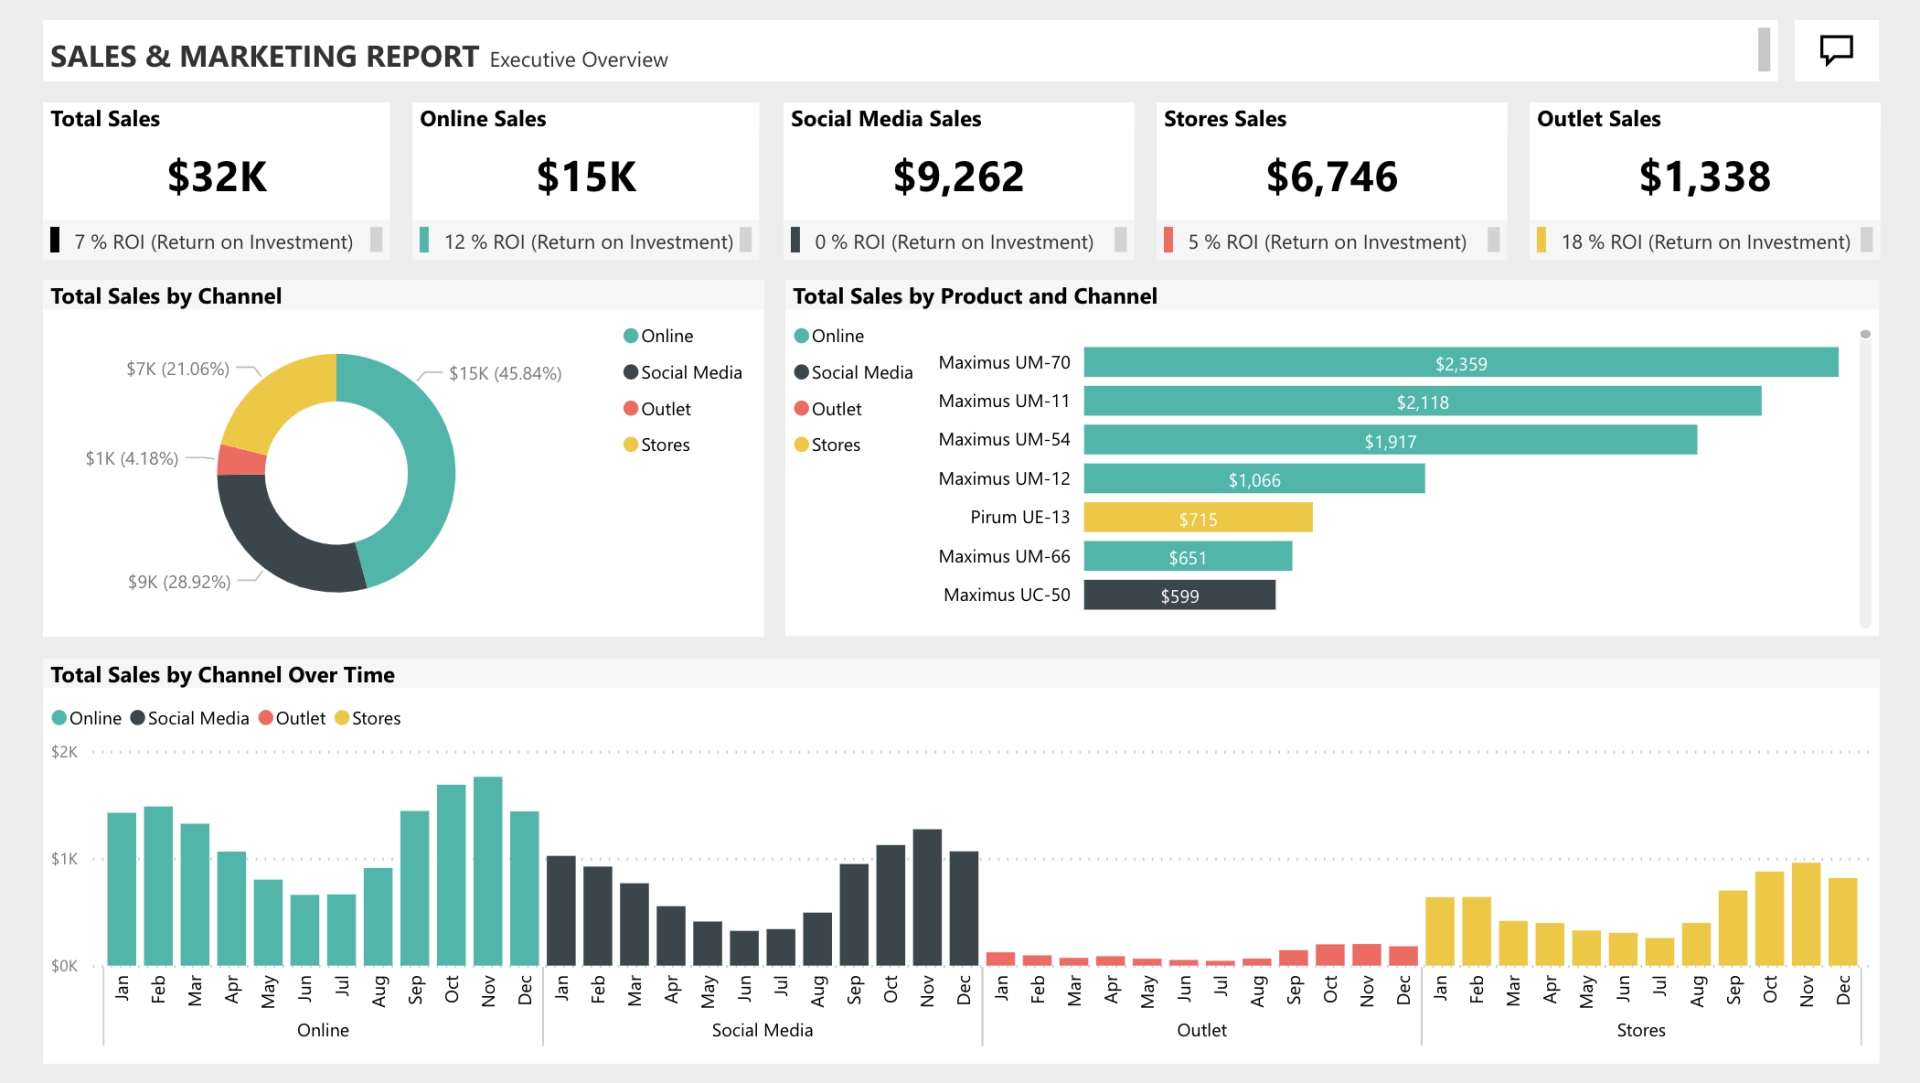
\includegraphics[width=0.7\textwidth]{images/power_bi_ejemplo.png} 
    \label{fig:subfig1}%
  }\hfill

  \subfloat[Ejemplo de uso de la función Natural Language Q \& A Question Box de \texttt{Power BI}.]{%
    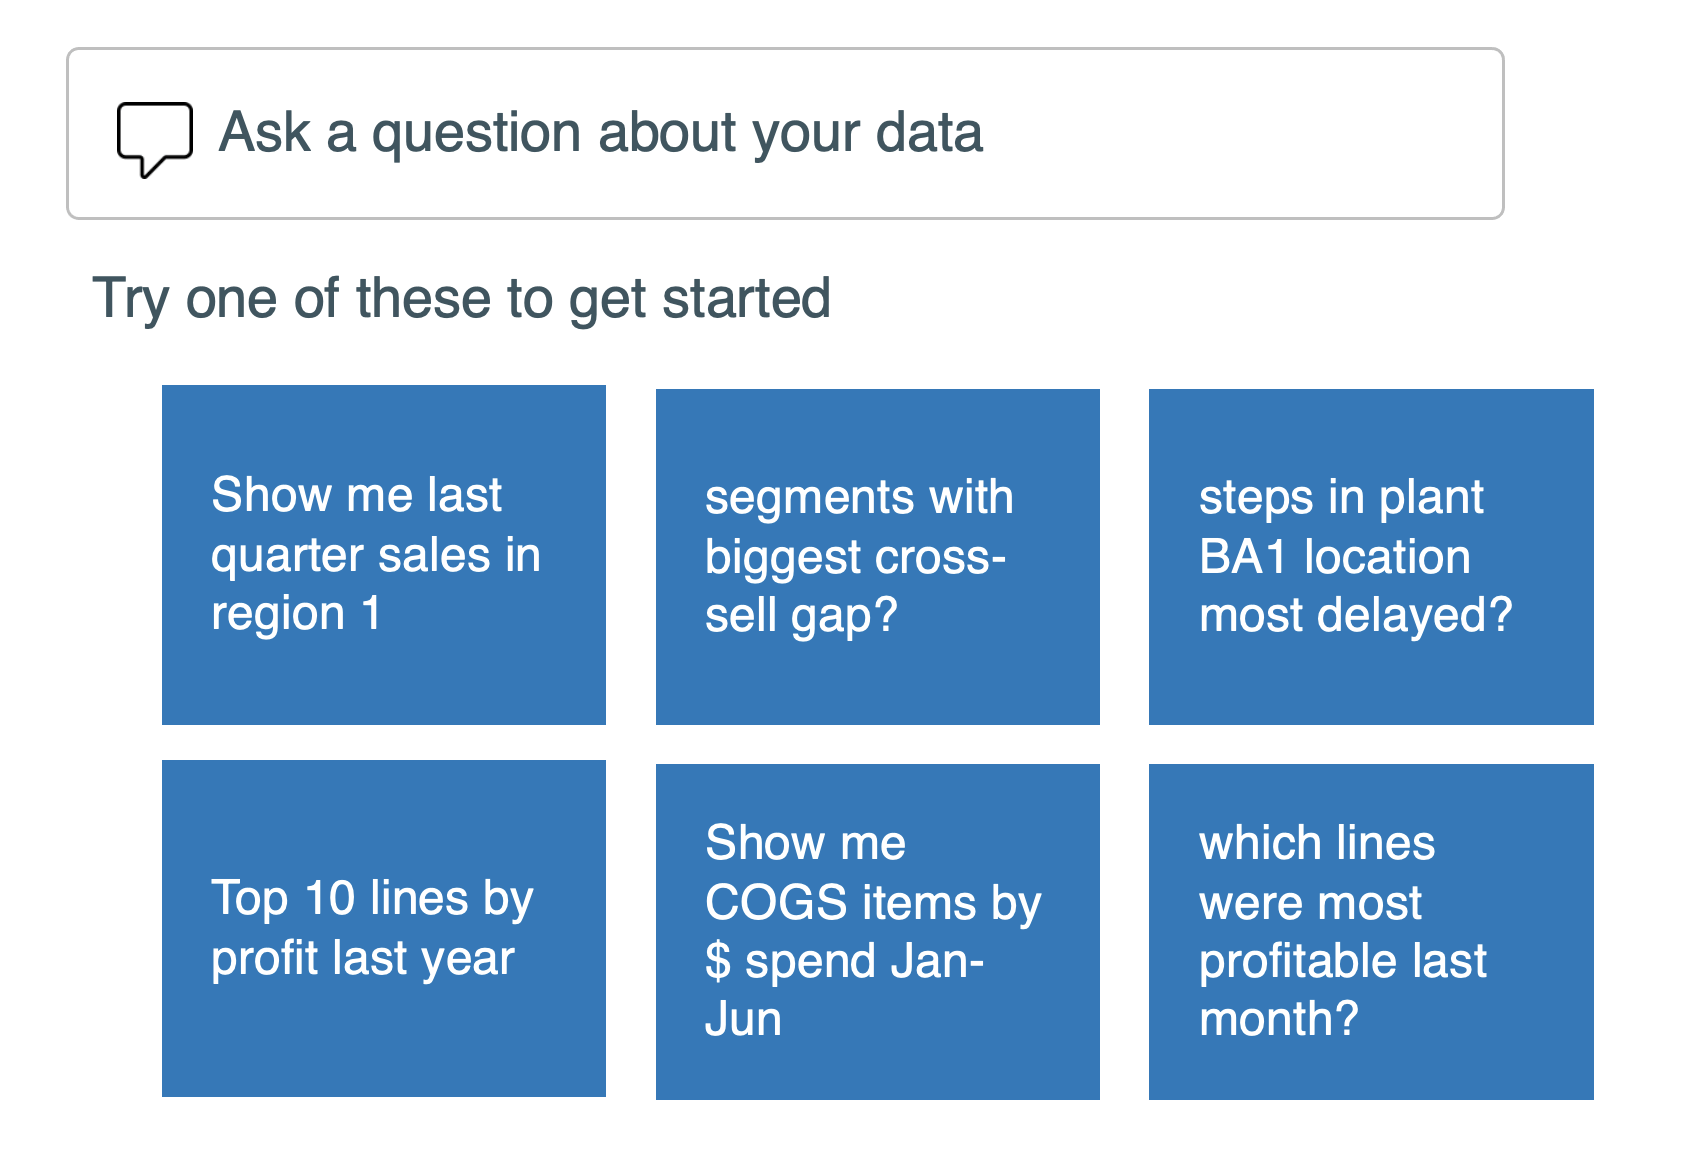
\includegraphics[width=0.7\textwidth]{images/power_bi_Q&A.png}
    \label{fig:subfig2}%
  }

  \caption{Ejemplos de uso de \texttt{Power BI}.}
  \label{fig:overall}
\end{figure}

Las razones por las cuales no se hizo uso de Power BI es debido a que en el proyecto no se tienen integrados productos de Microsoft mas que GitHub, lo cual no le quita valor a todo lo que Power BI ofrece, pero se podría hacer un uso más provechoso si en el proyecto se trabajara con un \textit{stack} más enfocado en productos de Microsoft como Azure. Además el costo por una licencia individual para un desarrollador va desde 211 hasta 422 pesos mexicanos, lo cual no es algo que verdaderamente convenga pagar para este tipo de proyecto y las licencias para organizaciones, su precio varias dependiendo de las necesidades. Por último, \textbf{SEDESA} solicitó que todos los módulos del proyecto se encuentren en un mismo sitio, es decir, que se puedan acceder de manera sencilla, por lo que tener únicamente el tablero en una plataforma diferente no es lo más apropiado dado los requerimientos del proyecto.

\subsection{Tableau}
Tableau es una herramienta líder de Business Intelligence (BI) y visualización de datos, diseñada para hacer que el análisis de datos sea accesible e intuitivo para usuarios de distintos niveles. Permite a individuos y organizaciones transformar datos en crudo en tableros de datos interactivos y compartibles, proporcionando información que impulsa la toma de decisiones informadas.\\
A diferencia de las herramientas para creación de tableros de datos, que requieren amplios conocimientos técnicos, Tableau busca dar prioridad a la facilidad de uso, lo que permite a los usuarios técnicos y no técnicos crear visualizaciones y análisis complejos con facilidad. Es compatible con una amplia gama de fuentes de datos, desde hojas de cálculo y bases de datos hasta servicios en la nube, lo que garantiza flexibilidad y conectividad.\\



Entre las caracteristicas de Tableau, se pueden encontrar las siguientes:
\begin{itemize}
    \item Tableau cuenta con más de 100 conexiones de datos integradas que van desde archivos de texto como Excel a bases de datos como PostgreSQL o herramientas en línea como Google Analytics o Salesforce.com.

    \item Tableau provee una interfaz amigable con el usuario basada únicamente en las acciones de arrastrar y soltar, la interfaz de usuario permite crear fácilmente cuadros, gráficos, mapas y otras visualizaciones sin necesidad de amplios conocimientos previos en programación.

    \item Los usuarios pueden crear visualizaciones dinámicas y atractivas que permiten a los espectadores explorar interactivamente los datos a través de filtros, capacidades de desglose y parámetros personalizables.

    \item Tableau proporciona funciones estadísticas incorporadas, como regresiones lineales, coeficientes de correlación y desviaciones estándar, lo que permite realizar análisis más avanzados dentro de la propia plataforma si es que así se desea.

    \item De manera similar a Power BI, Tableau también ofrece un función que usa procesamiento de lenguaje natural para hacer preguntas sobre los conjuntos de datos que se manipula.

    \item La función que podría ser considera la más útil y atrayente de Tableau, es el poder combinar datos de diferentes. Por ejemplo, combinar datos que se encuentran contenidos en un hoja de calculo de Excel y diferentes datos que se encuentran en PostgreSQL.

    Existen varias formas de combinar datos, cada una con sus propios puntos fuertes y débiles.

    \begin{itemize}
        \item Las relaciones son el método por defecto y pueden utilizarse en la mayoría de los casos, incluso entre tablas con distintos niveles de detalle.

        \item Las uniones combinan tablas añadiendo más columnas de datos a través de estructuras de filas similares. Esto puede provocar la pérdida o duplicación de datos si las tablas tienen diferentes niveles de detalle.

        \item Las mezclas, a diferencia de las relaciones o las uniones, nunca combinan los datos directamente. En su lugar, las mezclas consultan cada fuente de datos de forma independiente, agregan los resultados al nivel adecuado y, a continuación, los presentan juntos visualmente en la vista. 
    \end{itemize}


    Como se puede observar Tableau es un software bastante poderoso que ofrece una amplia gama de herramientas y facilidades para la implementación de tableros datos y distintas visualizaciones.\\
    Es una excelente herramienta que se pudo haber utilizado para el desarrollo de este trabajo, pero como se mencionó en el primer capitulo los recursos asignados para la compra de software de pago es limitado y Tableau cuenta con precios de licencias por desarrollador elevados los cuales van desde los 15 hasta los 75 dolares mensuales. De manera similar a lo mencionado anterior anteriormente con Power BI, todos los módulos solicitados por \textbf{SEDESA}, los cuales no se limitan solamente a la visualización de datos, deben estar localizados dentro una misma aplicación o software.

\end{itemize}




\section{Resumen}
En esta capítulo se resumen las técnicas y métodos que han sido desarrollados hasta el momento para ....
 
 
